\subsection{实验目的}
理解集成学习的概念和评价分类器性能的评价方法,掌握一些典型的集成学习方法和分类器性能评价方法,例如Bagging方法。完成遥感图像的图像分类。
\subsection{实验原理}
\begin{description}
	\item[集成学习] 原理:构建并结合多个学习器来完成学习任务,提升泛化性能。
	\begin{figure}[H]
		\centering
		\begin{tikzpicture}[node distance=1.5cm]
		\node(classifier_1) [process] {个体学习器1};
		\node(classifier_2) [process, below of=classifier_1] {个体学习器2};
		\node(dots) [empty_process, below of=classifier_2] {$\vdots$};
		\node(classifier_3) [process, below of=dots] {个体学习器n};
		\node(combination) [process, right of=classifier_2, node distance=5cm] {结合模块};
		\node(output_classification) [io, right of=combination, node distance=5cm] {输出};
		
		\draw[arrow] (classifier_1) -- (combination);
		\draw[arrow] (classifier_2) -- (combination);
		\draw[arrow] (classifier_3) -- (combination);
		\draw[arrow] (combination) -- (output_classification);
		\end{tikzpicture}
	\end{figure}
	\item[个体学习器] 从训练数据学习的一个分类器,比如线性判别函数。个体学习器应好而不同。
	\item[Bagging方法] 思想:通过对训练数据集采样,得到不同的子集,每个子集训练一个个体学习器,使用相互交叠的子集。\\
	自助取样法:随机取出一个样本放入采样集,再把该样本放回初始数据集,使得下次采样时仍可能选中该样本。
	\item[集成学习——投票法] 对于一个数据进行分类,在不同学习器中可以会出现不同的分类结果。对于这种情况,这个数据最终的分类服从“少数服从多数”的原则,即采纳得到票数最高的分类判定。
\end{description}
\subsection{实验流程}
\begin{figure}[H]
	\centering
	\begin{tikzpicture}[node distance=1.5cm]
	\node(begin) [startstop] {开始};
	\node(input_img) [io, below of=begin] {读取待分类的图片};
	\node(abstracting_training_set) [process, below of=input_img] {提取训练样本};
	\node(generate_negative_training_set) [process, below of=abstracting_training_set] {生成负样本集};
	\node(sample_training_set) [process, below of=generate_negative_training_set] {抽取产生多个学习器使用的训练样本};
	\node(training_classifiers) [process, below of=sample_training_set] {训练多个学习器};
	\node(voting) [process, below of=training_classifiers] {投票产生最终的分类结果};
	\node(calculating_accuracy) [process, below of=voting] {计算正确率};
	\node(output_classification) [io, below of=calculating_accuracy] {输出显示分类结果};
	\node(end) [startstop, below of=output_classification] {结束};
	
	\draw[arrow] (begin) -- (input_img);
	\draw[arrow] (input_img) -- (abstracting_training_set);
	\draw[arrow] (abstracting_training_set) -- (generate_negative_training_set);
	\draw[arrow] (generate_negative_training_set) -- (sample_training_set);
	\draw[arrow] (sample_training_set) -- (training_classifiers);
	\draw[arrow] (training_classifiers) -- (voting);
	\draw[arrow] (voting) -- (calculating_accuracy);
	\draw[arrow] (calculating_accuracy) -- (output_classification);
	\draw[arrow] (output_classification) -- (end);
	\end{tikzpicture}
\end{figure}
\subsection{实验程序}
\lstinputlisting[caption={集成学习和正确率分析}]{"../Executable Script/Exp 6/EnsembleLearning.m"}
\lstinputlisting[caption={绘制矩形函数}]{"../Function Library/DrawRectangle.m"}
\lstinputlisting[caption={LDA分类器训练函数}]{"../Function Library/LDAClassification.m"}
\lstinputlisting[caption={LDA分类器生成分类逻辑函数}]{"../Function Library/LDAClassificationLogicMap.m"}
\lstinputlisting[caption={正确率计算函数}]{"../Function Library/ImageClassificationAccuracyJudgement.m"}
\subsection{实验结果和分析}
选择如图\ref{fig:airport_44_samples}所示的两块区域的数据作为训练样本,对学习器进行训练。
\begin{figure}[H]
	\centering
	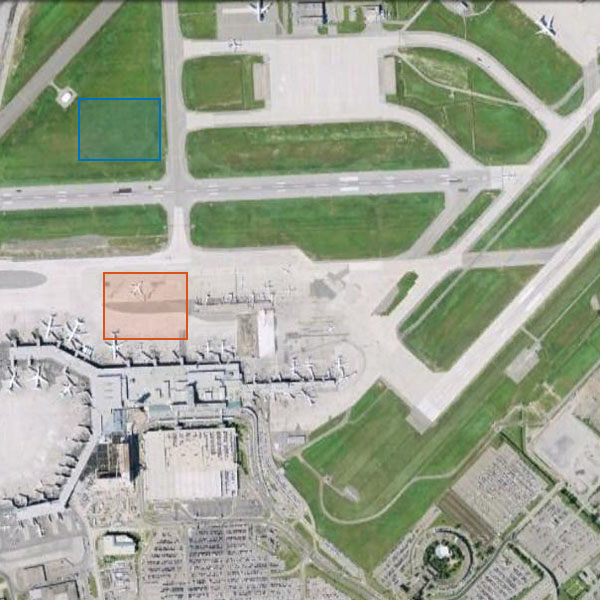
\includegraphics[width=0.7\linewidth]{figure/airport_44_Ensemble_Learning_Training_Set.png}
	\caption{训练样本的选取}
	\label{fig:airport_44_samples}
\end{figure}
对三个学习器进行训练,最终可以得到如下图所示的分类结果(白色区域代表该区域属于这个分类)。
\begin{figure}[H]
	\centering
	\begin{minipage}{0.45\linewidth}
		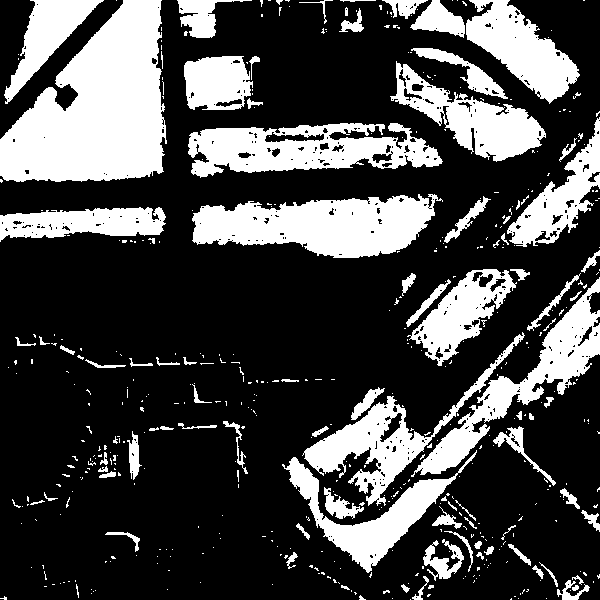
\includegraphics[width=\linewidth]{figure/airport_44_Classifier_1_Class_1.png}
		\caption{学习器1对分类1的分类结果}
	\end{minipage}
	\begin{minipage}{0.45\linewidth}
		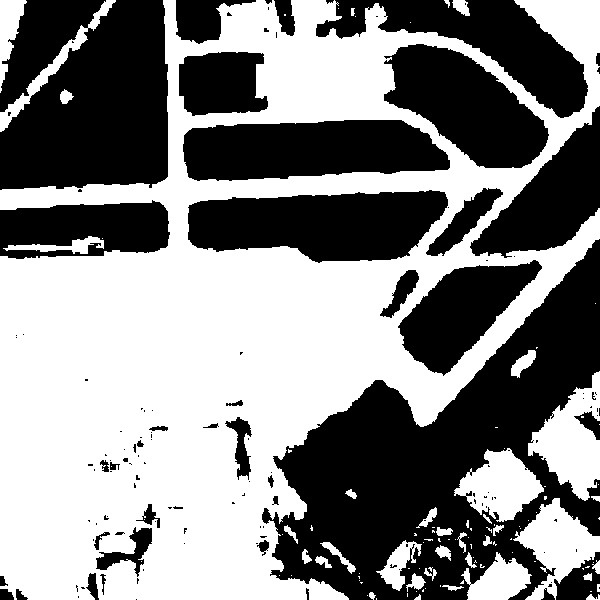
\includegraphics[width=\linewidth]{figure/airport_44_Classifier_1_Class_2.png}
		\caption{学习器1对分类2的分类结果}
	\end{minipage} \\
	\begin{minipage}{0.45\linewidth}
		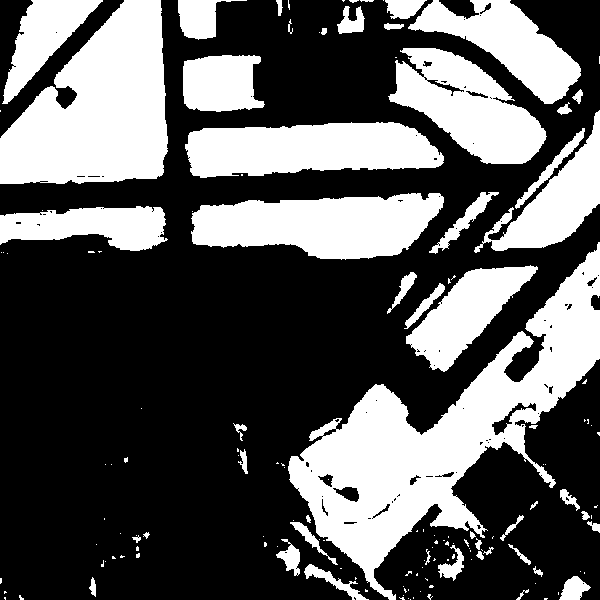
\includegraphics[width=\linewidth]{figure/airport_44_Classifier_2_Class_1.png}
		\caption{学习器2对分类1的分类结果}
	\end{minipage}
	\begin{minipage}{0.45\linewidth}
		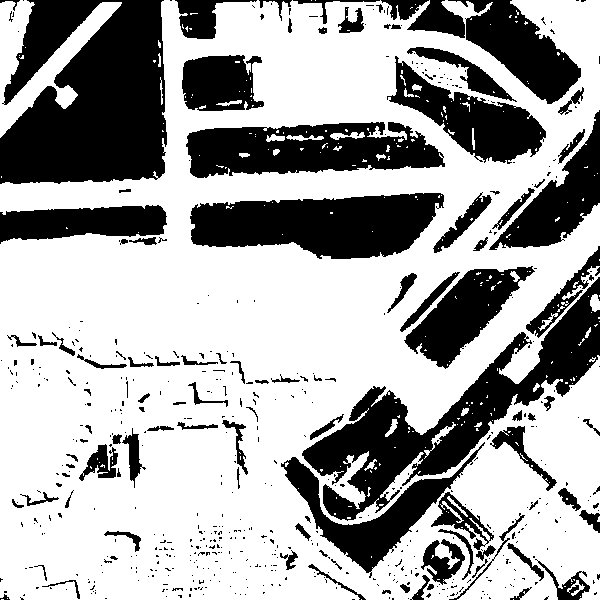
\includegraphics[width=\linewidth]{figure/airport_44_Classifier_2_Class_2.png}
		\caption{学习器2对分类2的分类结果}
	\end{minipage} \\
	\begin{minipage}{0.45\linewidth}
		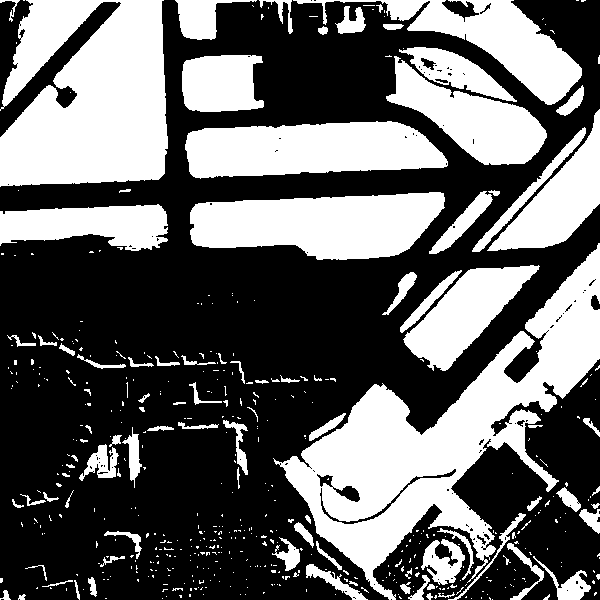
\includegraphics[width=\linewidth]{figure/airport_44_Classifier_3_Class_1.png}
		\caption{学习器3对分类1的分类结果}
	\end{minipage}
	\begin{minipage}{0.45\linewidth}
		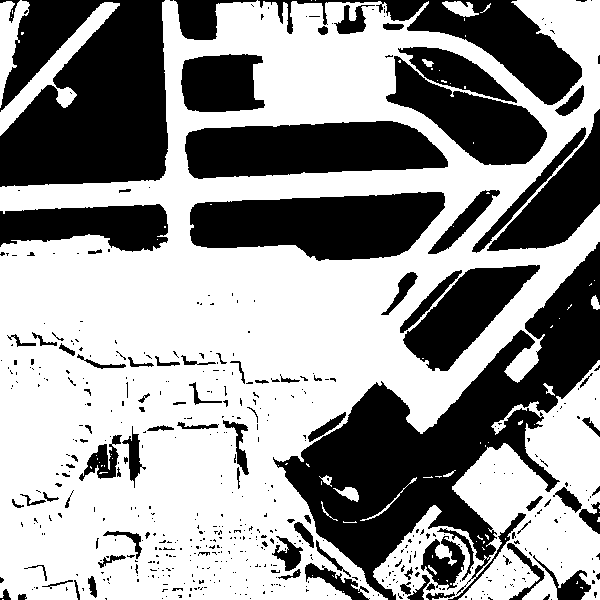
\includegraphics[width=\linewidth]{figure/airport_44_Classifier_3_Class_2.png}
		\caption{学习器3对分类2的分类结果}
	\end{minipage} 
\end{figure}
采用投票法对三个不同的学习器的分类结果进行合并,可以得到如下图所示的分类结果。
\begin{figure}[H]
	\centering	\begin{minipage}{0.45\linewidth}
		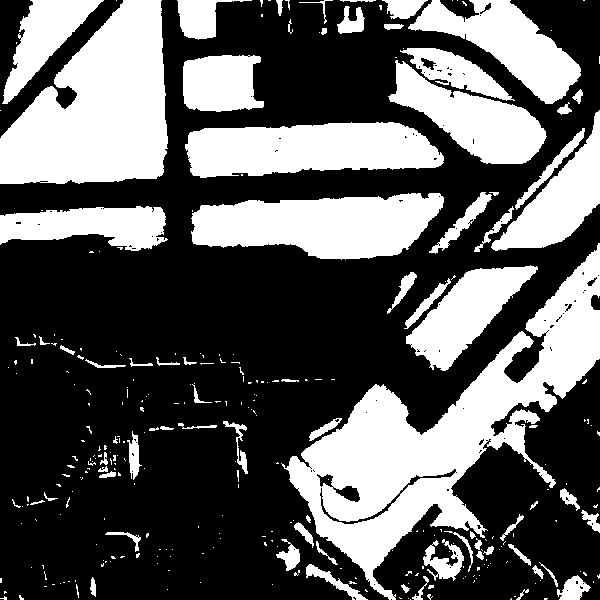
\includegraphics[width=\linewidth]{figure/airport_44_Class_1.png}
		\caption{分类1的分类结果}
	\end{minipage}
	\begin{minipage}{0.45\linewidth}
		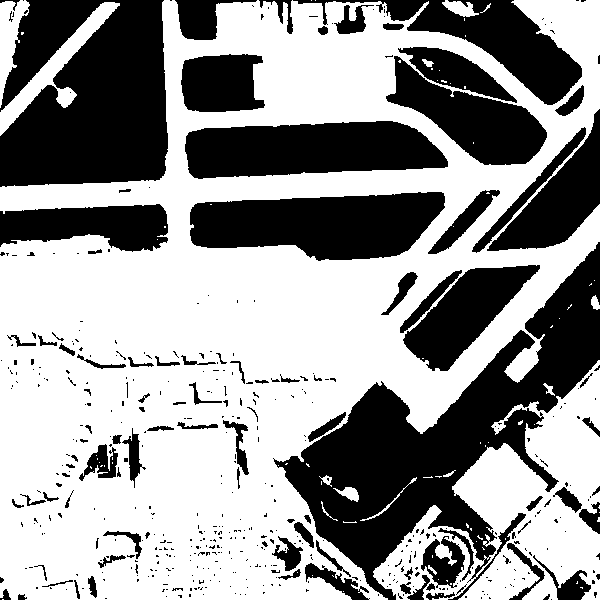
\includegraphics[width=\linewidth]{figure/airport_44_Class_2.png}
		\caption{分类2的分类结果}
	\end{minipage}
\end{figure}
对不同分类器的分类结果进行分析,可以得到它们的正确率,如下表所示。\\
\begin{tabular}{ccccc}
	\toprule
	算法 & 分类1 & 分类2 & 总正确率 & 平均正确率 \\
	\midrule
	分类器1 & 77.17\% & 86.45\% & 82.92\% & 82.92\% \\
	分类器2 & 97.40\% & 99.87\% & 98.93\% & 98.93\% \\
	分类器3 & 99.89\% & 99.71\% & 99.82\% & 99.82\% \\
	集成学习 & 97.32\% & 99.10\% & 98.84\% & 98.21\%  \\
	单个分类器 & 93.87\% & 94.20\% & 94.05\% & 94.04\% \\
	\bottomrule
\end{tabular}

从集成学习和分类的结果中分析,可以发现,由于线性判别函数的初始状态不同、训练样本不同,会导致最终的分类结果会有所不同,产生不确定性。而集成学习可以通过比较和处理来自不同分类器的分类结果,从而改善分类的效果,使分类的结果更加细致,减小不确定性。在多次尝试中,我发现选取的训练样本越多、分类器的数量越多,越能减小分类结果的不确定性,改善最终的分类结果,与此同时带来的代价就是要使用更多的计算资源和时间来对数据进行分类。